%
%

%%-----------------------------------------------------
%%-----------------------------------------------------
\usebackgroundtemplate{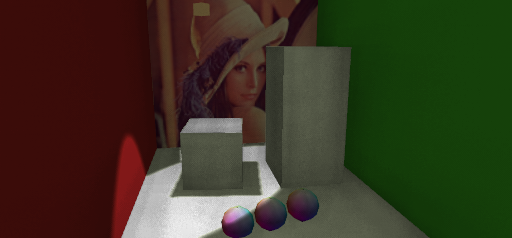
\includegraphics[width=\paperwidth,height=\paperheight]{figs/webgl-cornellbox}}
% Original figure: ``3D image of Cornell Box scene made with WebGL''
% from StormEngineC 3D Library
% License:  GNU Free Documentation License, Version 1.2 or later
% https://commons.wikimedia.org/wiki/File:WebGL_Cornell_Box.png
{\bf
  \textcolor[rgb]{1,1,1}{
    \section{Navegar en tres dimensiones}
  }
}

\usebackgroundtemplate{}

%%-----------------------------------------------------
\begin{frame}
\frametitle{WebGL}

\begin{columns}[T]
  \begin{column}{.40\textwidth}
    
\includegraphics[width=5.5cm]{figs/webgl-logo}
    \vspace{2cm}
    {\Large
      Mantenido por el Khronos Group
    }
  \end{column}%
  \hfill%
  \begin{column}{.58\textwidth}
    {\Large
      \begin{itemize}
      \item API JavaScript para gráficos interactivos en 3D
      \item Primeros desarrollos por Mozilla
      \item Proporcionada por los principales navegadores
      \item Puede mezclarse con HTML
      \item Basado en OpenGL
      \end{itemize}
    }
  \end{column}%
\end{columns}

\end{frame}

%%-----------------------------------------------------
\begin{frame}
\frametitle{Bibliotecas y utilidades}

{\Large
\begin{itemize}
\item API alto nivel: three.js, babylon.js
\item Motores de juegos: Unreal 4, Unity 5
\item Creación de escenas: Blender con Blend4Web, Clara.io
\end{itemize}
}
\vspace{1cm}
\begin{flushright}
  \url{http://threejs.org/} \\
  \url{http://babylonjs.com/} \\
  \url{https://blend4web.com/} \\
\end{flushright}
\end{frame}

%%-----------------------------------------------------
\begin{frame}
\frametitle{Algunos ejemplos}

{\Large
  \begin{itemize}
    \item Cube \\
    \url{http://www.playmapscube.com/} \\
  \item Experience Curiosity (Blend4Web)\\
    \url{http://eyes.nasa.gov/curiosity/} \\
  \item Sponza demo (babylon.js) \\
    \url{http://www.babylonjs.com/Demos/Sponza/} \\
  \item Above the clouds (three.js) \\
    \url{http://earth.plus360degrees.com/} \\
  \end{itemize}
}

\end{frame}


%%-----------------------------------------------------
\begin{frame}
\frametitle{Referencias y enlaces}

\begin{flushright}
  WebGL en Wikipedia \\
  \url{https://en.wikipedia.org/wiki/WebGL} \\
  \vspace{.5cm}
  WebGL en Mozilla Developer Network \\
  \url{https://developer.mozilla.org/en-US/docs/Web/API/WebGL_API} \\
  \vspace{.5cm}
  ``3D image of Cornell Box scene made with WebGL'', \\
  from StormEngineC 3D Library, GFDL 1.2 \\
  \url{https://commons.wikimedia.org/wiki/File:WebGL_Cornell_Box.png} \\
  \vspace{.5cm}
  ``WebGL tutorial'', by Mozilla \\
  \url{https://developer.mozilla.org/en-US/docs/Web/API/WebGL_API/Tutorial} \\
\end{flushright}  

\end{frame}






